\section{Aufbau und Durchführung}
\subsection{Verwendete Elemente}
Für den Versuch steht ein Optischer Tisch zur Verfügung, auf dem verschiedene Elemente montiert werden können. Dabei wird ein wie in \autoref{sec:Theorie} beschriebener Diodenlaser mitsamt Schutzabdeckung verwendet.
Außerdem ist eine Absorbtionszelle mit Rubidium, welche in einem Helmholtzspulenpaar montiert ist, sowie zwei Photodioden, ein Spektrometer und ein $50/50$-Strahlteiler vorhanden. Es liegt ebenfalls ein Mulitmeter zur 
Messung der Spannung am Thermoresistor und an der Diode bereit, sowie eine Tabelle, mit der die Spannung am Thermoresistor in die entsprechende Temperatur übersertzt werden kann. Außerdem stand ein Inbusschlüssel 
zur Verfügung, um die Feinjustierung des Lasers zu erleichtern.\\
\\
Der Laser 
und die Photodioden sind an ein Kontrollmodul angeschlossen. Über dieses lässt sich der an der Laserdiode anliegende Strom mit einer Genauigkeit von $\pm\qty{0.01}{\volt}$, 
die Temperatur der Laserdiode, Frequenz und Stärke eines Piezo-Elements
sowie ein Rampengenerator, der eine Dreiecksspannung erzeugt, steuern. Mit letzteren beiden lässt sich der Winkel des Beugungsgitters so modulieren, dass der Laser kontinuierlich durch verschiedene Frequenzen läuft. Das Signal der Photodiode
lässt sich nach einem Tiefpass über einen Ausgang abnehmen. Dieser kann, neben dem Ausgang des Rampengenerators und Piezo-Elements an ein Zwei-Kanal-Oszilloskop angeschlossen werden. \\
\\
Zusätzlich
steht eine Infrarot-Sichtkarte (IR-Sichtkarte) sowie eine Kamera, die an einen Monitor angeschlossen ist, zur Verfügung, um den Strahlengang des Lasers verfolgen zu können und die Floureszenz des Rubidiums zu beobachten.
Zu diesem Zweck hat die Ummantelung Rubidiumzelle ein Sichtfenster, an welches die Kamera gestellt werden kann. Darüber hinaus 
stehen bereits die BNC-Kabel zum Verbinden der Ein- und Ausgänge des Oszilloskops und des Kontrollmoduls sowie Halterungen für den Strahlteiler und die Sichtkarte zur Verfügung.

\subsection{Justierung des Lasers}

Zunächst muss der Diodenlaser zum in den Laser-Betrieb geschaltet und eine der diskreten Moden mit einer der größten Intensitäten gefunden werden. Dabei wird als Erstes überprüft ob die Diodenspannung am Kontrollmodul
ausgeschaltet ist. Daraufhin kann dann der Hauptschalter am Kontrollmodul betätigt werden. 
\subsubsection{Finden einer der Moden mit größter Intensität}
\label{sec:durch1}
Nun muss die Temperatur am Diodenchip auf den gewünschten Wert voreingestellt werden. Dazu wird das Multimeter, welches in \autoref{fig:multimeter} zu sehen ist, an den entsprechenden Ausgang des Thermoresistors am Kontrollmodul angeschlossen und auf einen
Messbereich von $\qty{2}{\volt}$ mit einer Unsicherheit von $\pm\qty{0.1}{\volt}$ eingestellt. Die Temperatur kann nun über einen Drehknopf auf der Rückseite des Kontrollmoduls eingestellt werden. Mithilfe der Tabelle kann nun die Temperatur initial auf 
$\qty{50}{\degreeCelsius}$ voreingestellt werden. Dabei ist allerdings zu beachten, dass das System eine gewisse Relaxationszeit hat, bis sich nach Drehen des Knaufes auf die neue Temperatur eingependelt hat. 
\begin{figure}
    \centering
    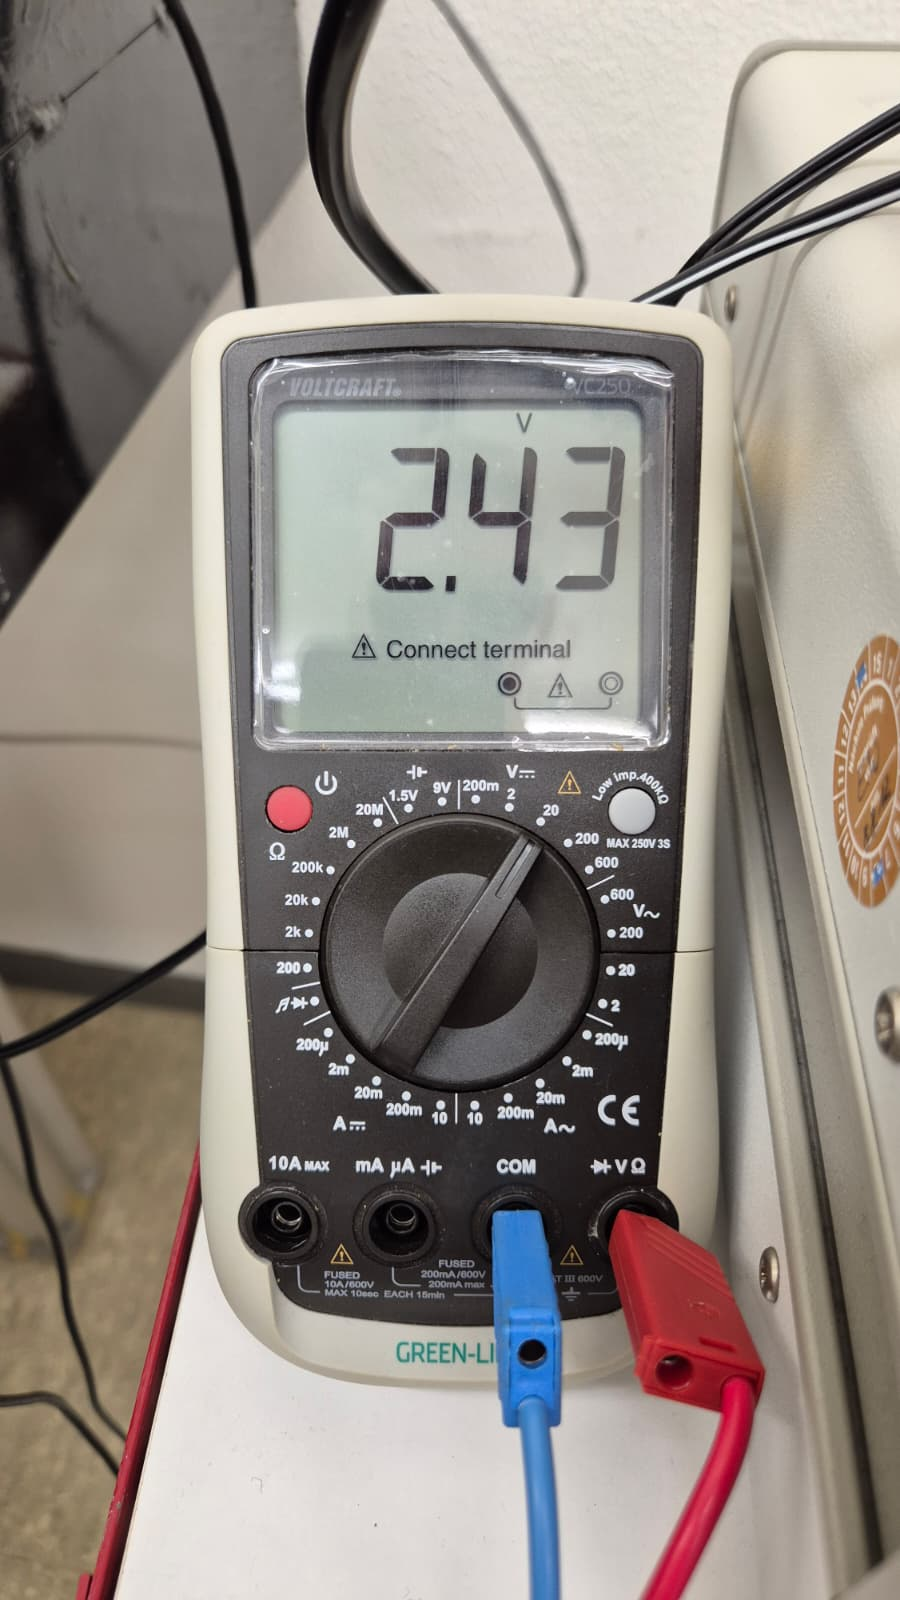
\includegraphics[width=0.3\textwidth]{content/images/multimeter.jpeg}
    \caption{An Kontrollmodul angeschlossenes Multimeter.}
    \label{fig:multimeter}
\end{figure}
\\
Im nächsten Schritt wird die Abdeckung des Lasers abgenommen und die IR-Sichtkarte vor dem Laser in einer Halterung eingespannt. Außerdem sollte die Kamera auf die Karte gerichtet werden, da 
der Laser mit bloßem Auge auf der Karte schwer zu erkennen ist. Nun kann langsam die Diodenspannung am Kontrollmodul erhöht werden, bis auf der Sichtkarte zu erkennen ist, dass die Diode in die
Phase der Laseraktivität übergegangen ist. Nun kann mithilfe des passenden Inbusschlüssels der obere Knopf am Laser, wie in \autoref{fig:diodenlaser} zu erknnen, gedreht werden. Dieser kontrolliert die vertikale Position des Gratings.
Es ist auf der Sichtkarte dabei zu erkennen, wie der Laser
mehrere Moden duchläuft, da seine Intensität schwankt. Dann sollte möglichst die Mode mit der größten Intensität gewählt werden. Nun wird die anliegende Spannung wieder runtergeregelt und auch der
obere Knopf am Laser ggf. erneut verstellt bis die Diode knapp oberhalb der Schwelle für die Erzeugung von Laserlicht ist. 
\begin{figure}
    \centering
    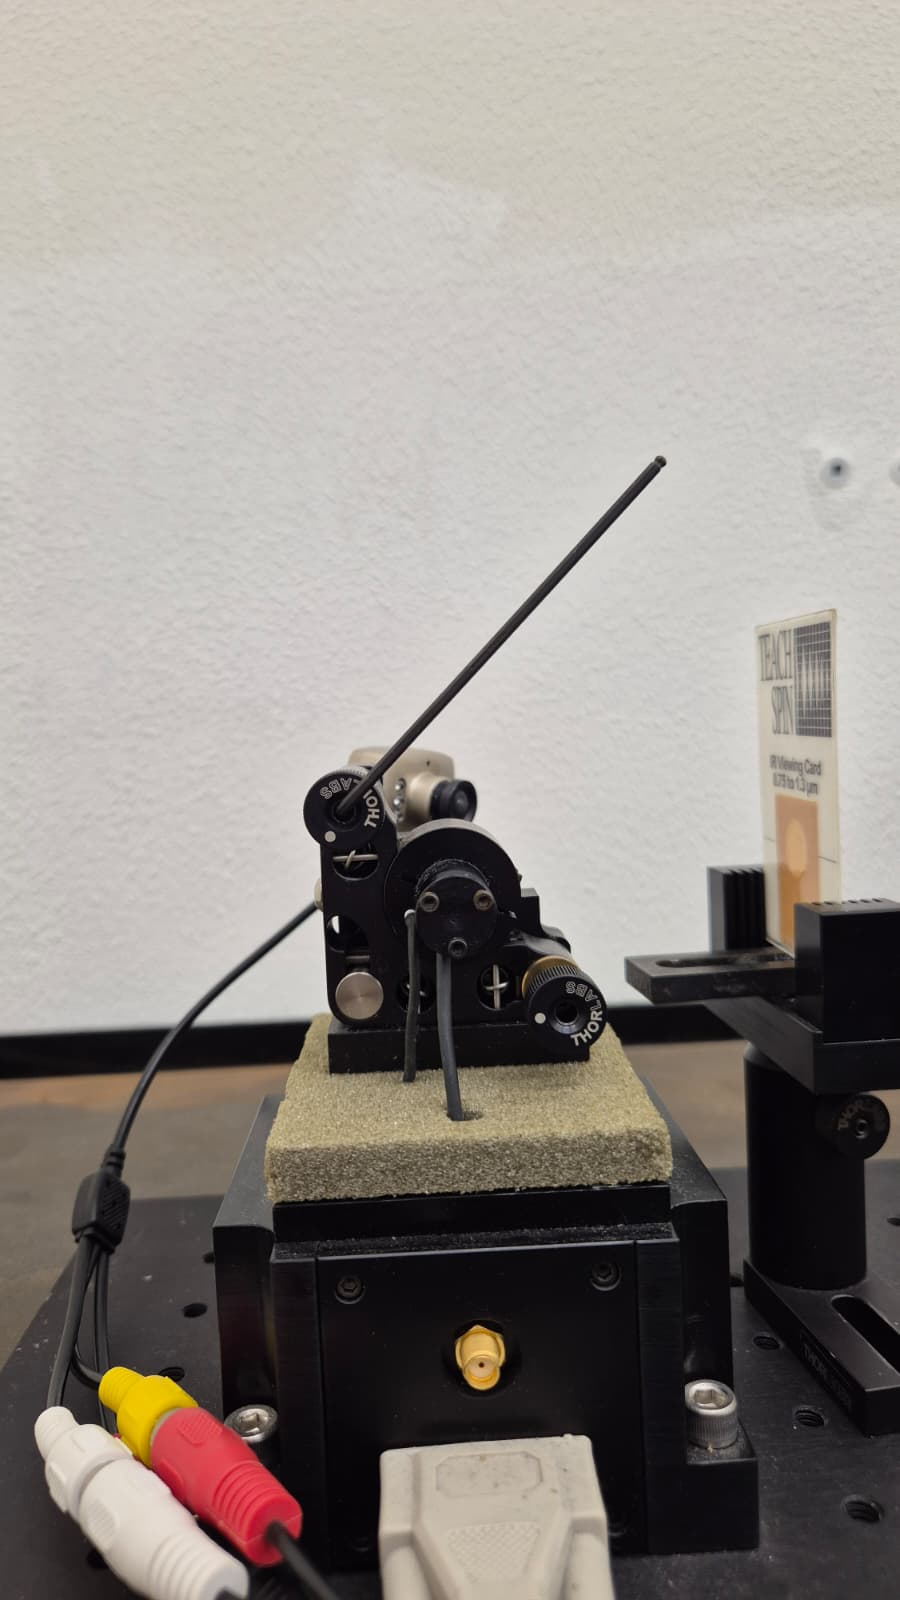
\includegraphics[width=0.3\textwidth]{content/images/diodenlaser.jpeg}
    \caption{Diodenlaser mit oberem Knopf (oben links, eingesteckter Imbusschlüssel) und unterem Knopf (unten rechts).}
    \label{fig:diodenlaser}
\end{figure}
\\
\subsubsection{Anpassung der Wellenlänge anhand von Rubidiumfloureszenz}
\label{sec:durch2}
Nach erfolgreicher vertikaler Justierung wird die Rubidiumzelle in den Strahlengang gestellt, sodass der Laserstrahl sie vollständig durchquert. Dazu kann die Sichtkarte aus der Halterung entnommen und zur Hilfe verwendet werden. 
Zudem wird vor der Rubidiumzelle ein 50/50 Strahlteiler mittels der Halterung in den Strahlengang gebracht. Der transmittierte Anteil geht dann durch die Zelle. In den Strahlengang des reflektierten Anteils wird
das Spektrometer eingebracht. Die Kamera sollte an das dafür vorgesehenne Sichtfenster in der Rubidiumzelle gestellt werden, um das Floureszenzlicht auf dem Monitor beobachten zu können.
Der Aufbau ist in \autoref{fig:tischdraufsicht} zu erkennen. 
\begin{figure}
    \centering
    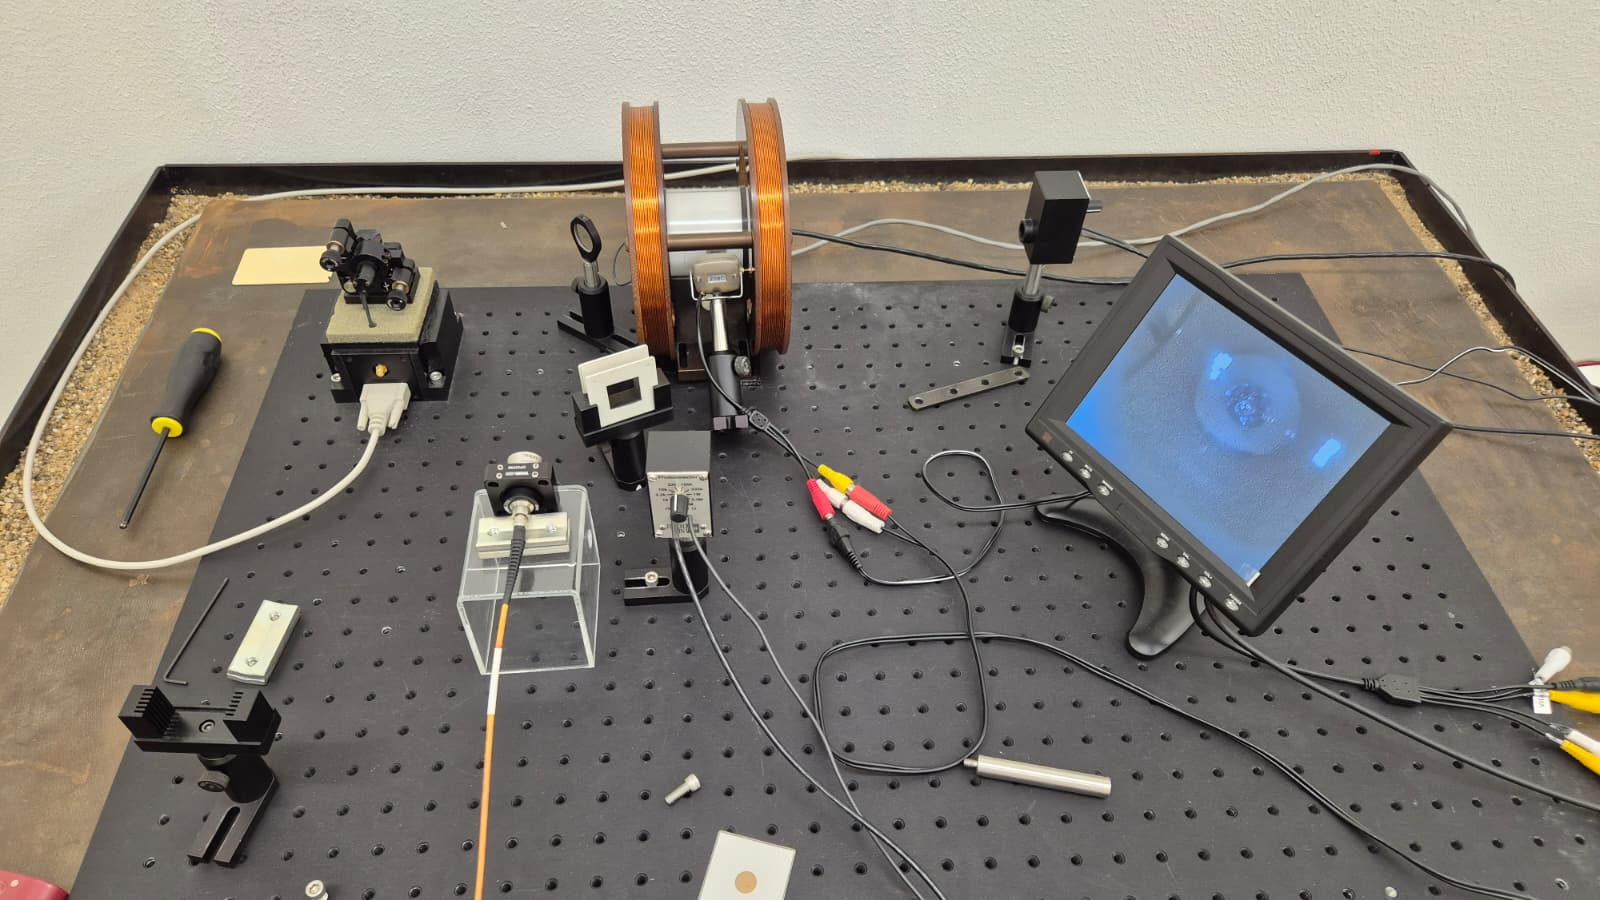
\includegraphics[width=0.5\textwidth]{content/images/tischdraufsicht.jpeg}
    \caption{Draufsicht auf den Tisch bei Aufbau für die Justierung der Wellenlänge.}
    \label{fig:tischdraufsicht}
\end{figure}
\\
Nun können beide Knöpfe am Laser, die anliegende Diodenspannung, sowie die Temperatur feinjustiert werden. Dabei wird zunächst wie folgt vorgegangen: Bei fester Temperatur und fester Spannung wird
zunächst der Seitliche Knopf in beide Richtungen jeweils um Maximal eine ganze Umdrehung gehdreht und dann wieder in die Ausgangspostion gebracht. Ist kein Floureszenzlicht zu sehen wird nun die 
Spannung um etwas $\qty{0.33}{\volt}$ erhöht und das Drehen des Knopfes wiederholt. Dabei lässt sich die Spannung maximal auf $\qty{8.43}{\volt}$ erhöhen. Ist weiterhin kein Floureszenzlicht zu sehen
wird der Prozess für eine andere Temperatur wiederholt. Diese wird dabei jeweils in $\qty{2}{\degreeCelsius}$ Schritten angepasst. Ist immer noch keine Floureszenz zu erkennen, wird das Spektrometer 
zur Hilfe genommen. Nun wird die Ausgabe des Spektrometers beobachtet und an allen vier Stellschrauben gedreht, bis die angezeigte Wellenlänge den gewünschten $\qty{780}{\nano\meter}$ der Rubidiumübergänge
möglichst nahe kommt. Das Spektrometer zeigt dabei einen deutlichen Peak bei der Welllenlänge des Lasers an. Anschließend
wird wieder der Monitor beobachtet und der Laser über die beiden Knöpfe weiter feinjustiert, bis auf dem Bildschirm das Floureszenzlicht zu sehen ist. 
\subsubsection{Durchscannen des Frequenzbereiches}
\label{sec:durch3}
Zunächst muss die Amplitude des Rampengenerators am Kontrollmodul sowie der Knopf \enquote{output offset} ausgeschaltet werden. Dann wird der Rampengenerator durch die BNC-Kabel mit dem Oszilloskop verbunden.
Nun wird am Rampengenerator eine Frequenz von $\qty{10}{\hertz}$, der Knopf \enquote{Attenuator} am Piezo-Element auf $1$ und die Amplitude des
Rampengenerators auf $10$ eingestellt. Mithilfe des Oszilloskops kann nun am Kopf \enquote{output offset} so justiert werden, bis eine Dreieckspannung, die oben und unten auf dem Bildschirm nicht abgeschnitten ist, zu erkennen ist. 
Nun werden die Elemente, wie in \autoref{fig:piezo} dargestellt, miteinander verbunden. Es wird überprüft ob, das Signal des Piezo-Elements nun im Bereich von 
$\qty{3}{\volt}$ bis $\qty{8}{\volt}$ liegt und gegebenenfalls nachjustiert. 
\begin{figure}
    \centering
    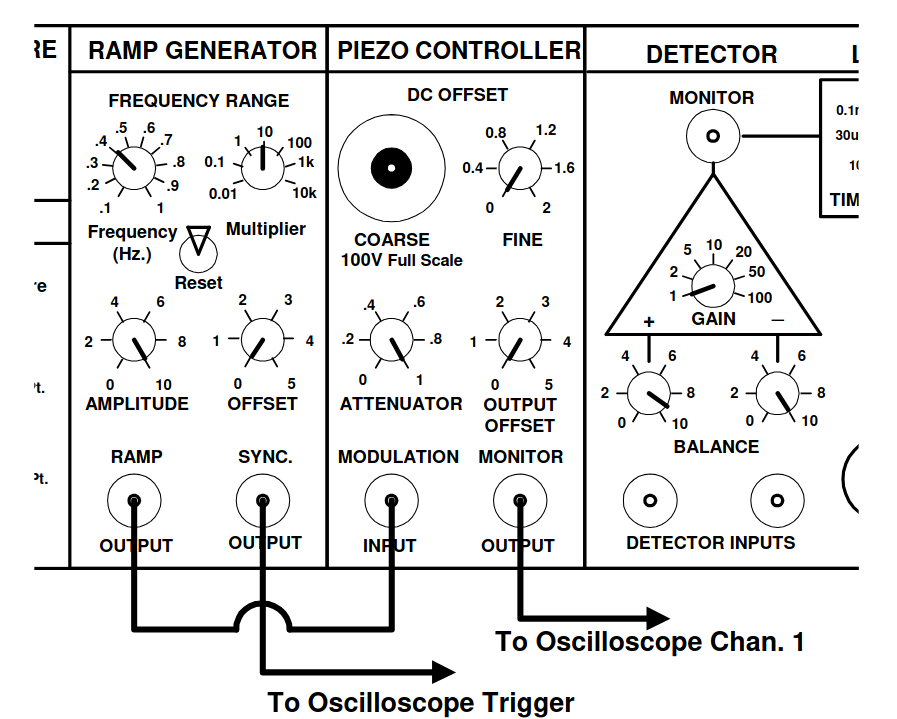
\includegraphics[width=0.7\textwidth]{content/images/piezoschaltung.png}
    \caption{Schamtische Schaltung für die Einstellung des Piezo-Elements und des Rampengenerators \cite{V60}.}
    \label{fig:piezo}
\end{figure}
\\
Als Nächstes wird hinter der Rubidiumzelle eine Photodiode, die mit dem Detektor-Eingang des Kontrollmoduls verbunden ist, in den Strahlengang der Lasers verbaut. Der Ausgang hinter dem Tiefpass 
wird nun mit dem zweiten eingang des Oszilloskops verbunden. Am Oszilloskop sind nun mehrere Absorbtionslinien des Rubidiums zu erkennen, da der Laser einen Frequenzbereich durchläuft. 
\label{sec:Durchführung}

